\documentclass{article}
\usepackage{graphicx}
\usepackage{float}
\usepackage{booktabs}
\usepackage{tikz}
\begin{document}
	
	\title{Regression Algorithms Assignment}
	\author{K.N.Toosi University of Technology\\Introduction to Data Mining}
	\date{Fall 2024}
	\maketitle
	\newpage
	\part{Practical Assignment:\\Linear Regression}
			\section*{Task}
			The objective of this assignment is to provide hands-on experience with fitting a linear regression model using given data points in Figure \ref{lr}. Students are asked to assess their model's accuracy using \textit{MSE} and solve for parameters $\alpha$ and $\beta$.
			\section*{Data Points}
			\begin{figure}[H]
			\begin{center}
				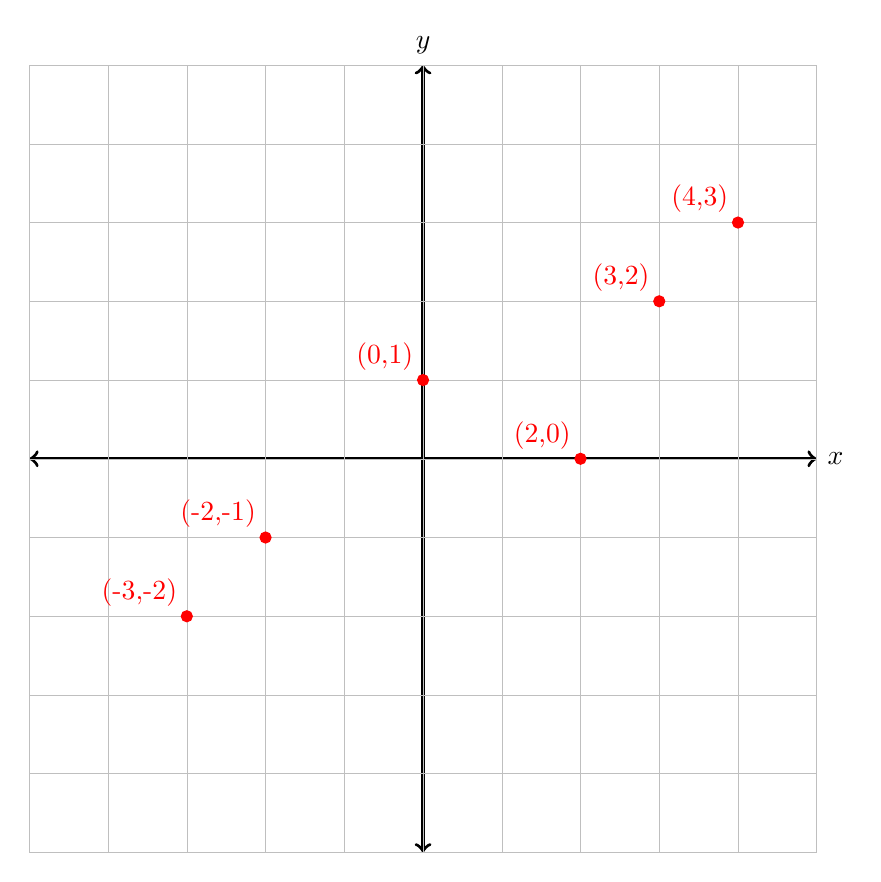
\begin{tikzpicture}
					% Draw the axes with thicker lines
					\draw[<->, very thick] (-5,0) -- (5,0) node[right] {$x$};
					\draw[<->, very thick] (0,-5) -- (0,5) node[above] {$y$};
					
					% Draw faded grid
					\draw[step=1cm,gray!50,very thin] (-5,-5) grid (5,5);
					
					% Plot the points
					\filldraw[red] (-3, -2) circle (2pt) node[anchor=south east] {(-3,-2)};
					\filldraw[red] (-2, -1) circle (2pt) node[anchor=south east] {(-2,-1)};
					\filldraw[red] (0, 1) circle (2pt) node[anchor=south east] {(0,1)};
					\filldraw[red] (2, 0) circle (2pt) node[anchor=south east] {(2,0)};
					\filldraw[red] (3, 2) circle (2pt) node[anchor=south east] {(3,2)};
					\filldraw[red] (4, 3) circle (2pt) node[anchor=south east] {(4,3)};
				\end{tikzpicture}
			\end{center}
				\caption{Linear Regression Data Points}
				\label{lr}
		\end{figure}
	\part{Practical Assignment:\\Polynomial Regression}
	\section*{Task}
	The goal of this assignment is to fit a 3rd degree polynomial function to the given set of data points in Figure \ref{pr} and report the resulting polynomial coefficients.
	\section*{Data Points}
	\begin{figure}[H]
		\begin{center}
			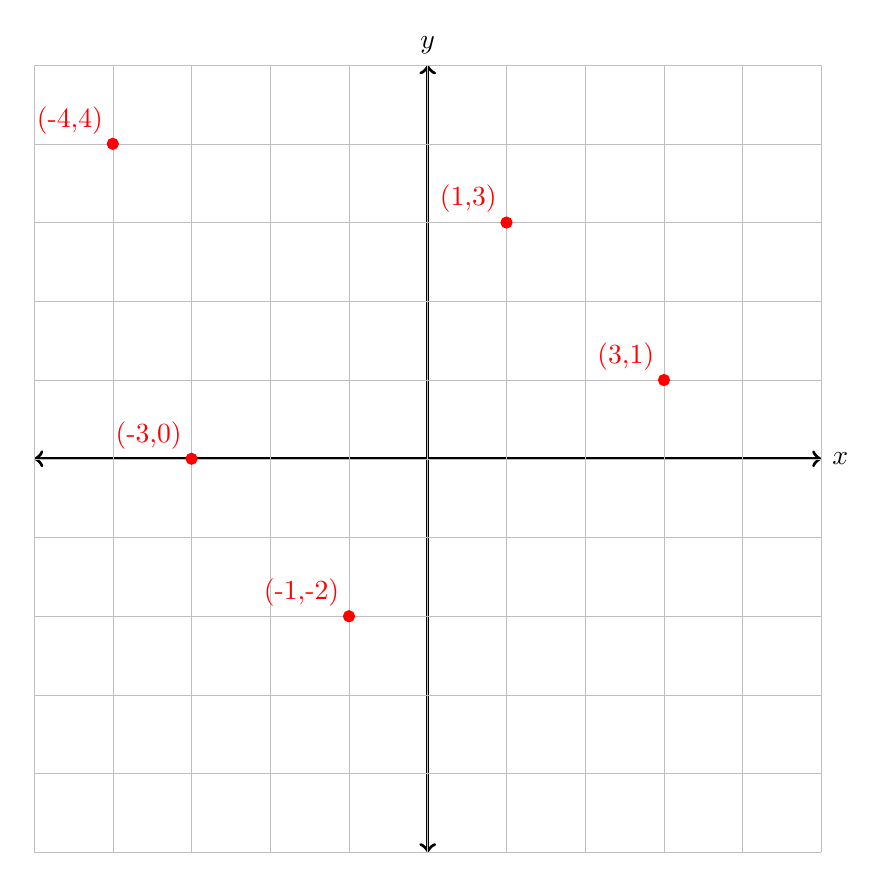
\begin{tikzpicture}
				% Draw the axes with thicker lines
				\draw[<->, very thick] (-5,0) -- (5,0) node[right] {$x$};
				\draw[<->, very thick] (0,-5) -- (0,5) node[above] {$y$};
				
				% Draw faded grid
				\draw[step=1cm,gray!50,very thin] (-5,-5) grid (5,5);
				
				% Plot the points
				\filldraw[red] (-4, 4) circle (2pt) node[anchor=south east] {(-4,4)};
				\filldraw[red] (-3, 0) circle (2pt) node[anchor=south east] {(-3,0)};
				\filldraw[red] (-1, -2) circle (2pt) node[anchor=south east] {(-1,-2)};
				\filldraw[red] (1, 3) circle (2pt) node[anchor=south east] {(1,3)};
				\filldraw[red] (3, 1) circle (2pt) node[anchor=south east] {(3,1)};
			\end{tikzpicture}
		\end{center}
		\caption{Polynomial Regression Data Points}
		\label{pr}
	\end{figure}
	\part{Implementation Assignment}
	\section*{Dataset}
	\begin{table}[h!] \centering \begin{tabular}{|c|c|} \hline \textbf{x} & \textbf{y (Label)} \\ \hline -4.5 & 0 \\ \hline -4 & 0 \\ \hline -3.5 & 0 \\ \hline -3 & 0 \\ \hline -2.5 & 0 \\ \hline -2 & 1 \\ \hline -1.5 & 1 \\ \hline -1 & 1 \\ \hline -0.5 & 1 \\ \hline 20 & 1 \\ \hline \end{tabular} \caption{Binary Classification Dataset} \label{T} \end{table}
	\section*{Task}
	This assignment aims to compare the flexibility and accuracy of logistic regression and linear regression in binary classification. You'll fit both models to the given dataset in Table \ref{T} using scikit-learn algorithms, visualize their decision boundaries, and analyze where linear regression falls short compared to logistic regression. Both models use a 0.5 threshold, and accuracy is measured by the number of correctly classified points.
	\section*{Note}
	Any attempt to use AI tools for generating the code is strictly prohibited. Students will be asked to present and explain their code during a class session.
\end{document}
